\documentclass[12pt,compress,aspectratio=169]{beamer}

\mode<presentation>
{
  \usetheme{Singapore}
  \setbeamersize{text margin left=1cm,text margin right=1cm}
%  \setbeamertemplate{navigation symbols}{} % suppress nav bar
%  \setbeamercovered{transparent}
}
\usefonttheme{professionalfonts}
\usepackage{amsmath,bm}
\usepackage{siunitx}
%\usepackage{graphicx}
\usepackage{tikz}
\usepackage{mathpazo}
\usepackage[scaled]{helvet}
\usepackage{xcolor,colortbl}
%\usepackage{hyperref}

\usetikzlibrary{decorations.pathmorphing,patterns}

\sisetup{number-math-rm=\mathnormal}

\title{Class 8: Gravitation}
\subtitle{AP Physics}
\author[TML]{Timothy Leung, Ph.D.}
\institute{Olympiads School}
\date{Fall/Winter 2017}

%\newcommand{\pic}[2]{\includegraphics[width=#1\textwidth]{#2}}
\newcommand{\mb}[1]{\ensuremath\mathbf{#1}}

\begin{document}

\begin{frame}
  \maketitle
\end{frame}


\begin{frame}
  \frametitle{Files to Download}
  \framesubtitle{Please download/print the PDF file}
%  If you have not done so already, please download the following files.
%  \begin{itemize}
%  \item\texttt{00-outline.pdf}--The slightly-updated course outline
%  \item\texttt{07-shm-print.pdf}--The ``print version'' of this week's
%    slides. I recommend printing 4 slides per page.
%  \item\texttt{07-Homework.pdf} This week's homework.
%  \end{itemize}
\end{frame}


\begin{frame}
  \frametitle{Today's Plan}
%  \begin{enumerate}
%  \item Take up (some) questions from Classes 4 and 5/6 homework
%  \item Go over this week's slides (hopefully it won't take too long)
%  \end{enumerate}
\end{frame}



\section{Gravitational Force}
%\begin{frame}
%  \frametitle{Hooke's Law}
%\end{frame}
%

\begin{frame}
  \frametitle{Gravitational Force}
%  \begin{itemize}
%  \item Consider the forces acting on a mass connected horizontally to a spring
  \begin{center}
    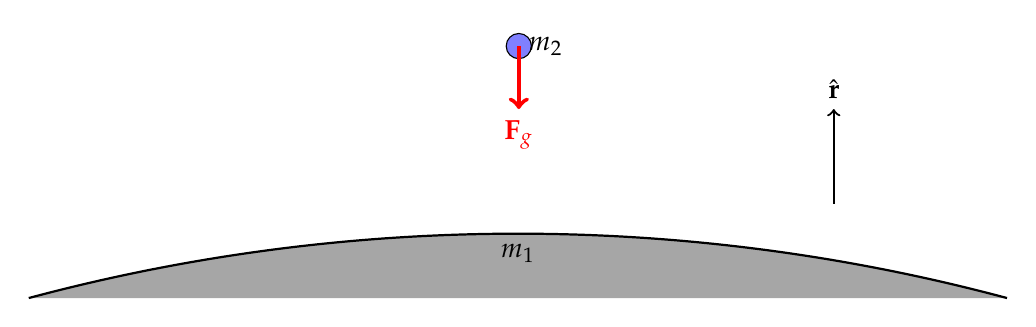
\begin{tikzpicture}[scale=0.8]
      \draw[thick,fill=gray!70] (7.75,0) arc(75:105:30)
      node[midway,below]{$m_1$};
      \draw[fill=blue!50] (0,4) circle(0.2) node[right]{$m_2$};
      \draw[ultra thick, red,->] (0,4)--(0,3)
      node[pos=1,below]{$\mb{F}_g$};
      \draw[->,thick](5,1.5)--(5,3) node[pos=1,above]{$\hat{\mb{r}}$};
    \end{tikzpicture}
  \end{center}
%  \item<3->$\mb{F}_g$ and $\mb{F}_N$ cancel out, so net force is due only to
%    spring force $\mb{F}_s=-k\mb{x}$. This is true both when the spring is in
%    compression or extension.
%  \item<4->Applying Newton's 2nd law in the $x$-direction, we get
%    
%  \vspace{-0.2in}

  {\Large
    \begin{displaymath}
      \mb{F}_g=-\frac{Gm_1m_2}{r^2}\hat{\mb{r}}
    \end{displaymath}
  }
%  \end{itemize}
\end{frame}



\section{Gravitational Potential Energy}


\begin{frame}
  \frametitle{Gravitational Potential Energy}

  \begin{itemize}
  \item The gravitrational potential energy is defined as:
    {\Large
      \begin{displaymath}
        \boxed{U_g=-\frac{Gm_1m_2}{r}}
    \end{displaymath}
    }
  %\item U_g is the work require to move two objects from $\inftypulled two objects apart, from a distance of
    % $r$ to $\infty$.
  \item It has a very similar form to the the equation for $\mb{F}_g$
  \item $U_g=0$ at $r=0$ and \emph{decrease} as $r$ decreases
  \end{itemize}
\end{frame}


\begin{frame}
  \frametitle{Relating Gravitational Potential Energy to Force}%{Relating $U_g$ and $\mb{F}_g$}% and $\mb{g}$}
  %\framesubtitle{It Helps to Know Calculus}
  \begin{itemize}
  \item If you know \emph{vector} calculus, you can easily see that
    gravitational force ($\mb{F}_g$) is the negative gradient of the
    gravitational potential energy ($U_g$):
    %through the gradient operator:
    %and gravitational field ($\mb{g}$) are related to

    \vspace{-0.1in}{\Large
      \begin{displaymath}
        \mb{F}_g=-\nabla U_g=
        -\frac{\partial U_g}{\partial r}\hat{\mb{r}}
        %\quad\;\;
        %\mb{g}=\nabla \left(\frac{U_g}{m}\right)=
        %-\frac{\partial}{\partial r}\left(\frac{U_g}{m}\right)
        %\hat{\mb{r}}
%        \quad\textrm{where}\quad
%        U_g=-\frac{Gm_1m_2}{r}
      \end{displaymath}
    }
  \item Even without using vector calculus, you should still see that, like
    all conservative force, $\Delta F_g=-\Delta U_g$, as we have seen in Class
    3
  \item The direction of $\mb{F}_g$ always points from high to low potential
    \begin{itemize}
    \item A falling object is always decreasing in $U_g$
    \item ``Steepest descent'': the direction of $\mb{F}$ is the shortest path
      to decrease $U_g$ 
    \item Objects traveling perpendicular to $\mb{F}$ has constant $U_g$
    \end{itemize}
  \end{itemize}
\end{frame}



%
%
%\begin{frame}
%  \frametitle{It's Very Ordinary}
%  \begin{itemize}
%  \item The governing equation for simple harmonic equation is an
%    \emph{ordinary differential equation}:
%
%    \vspace{-0.3in}{\Large
%      \begin{displaymath}
%        \boxed{\frac{d^2x}{dt^2}+\frac{k}{m}x=0}
%      \end{displaymath}
%    }
%  \item Starting with our general form, we can take the 1st and 2nd derivatives:
% 
%    \vspace{-0.35in}{\Large
%      \begin{align*}
%        x(t)&=A\sin(\omega t+\phi)\\
%        x'(t)&=A\omega\cos(\omega t+\phi)\\
%        x''(t)&=-A\omega^2\sin(\omega t+\phi)=-\omega^2x
%      \end{align*}
%    }
%    
%    \vspace{-0.2in}$\omega$ is the angular velocity, and $A$ is the amplitude,
%    and $\phi$ is a phase shift that depends on the initial condition of the
%    spring-mass system
%  \end{itemize}
%\end{frame}
%
%
%\begin{frame}
%  \frametitle{Mass on a Spring}
%  \framesubtitle{Angular Velocity}
%  \begin{itemize}
%  \item Substituting expressions of $x(t)$ and $x''(t)$ into the ODE, we find
%    our equation is satisfied if angular velocity (angular frequency) is:
%
%    \vspace{-0.2in}{\Large
%      \begin{displaymath}
%        \boxed{\omega=\sqrt{\frac{k}{m}}}
%      \end{displaymath}
%    }
%  \item Angular velocity $\omega$ does not depend on amplitude $A$
%
%  \item The period $T$ and frequency $f$ of the motion are given by:
%
%    \vspace{-0.2in}{\Large
%      \begin{displaymath}
%        \boxed{f=\frac{1}{2\pi}\sqrt{\frac{k}{m}}}\quad\quad\quad
%        \boxed{T=\frac{1}{f}=2\pi\sqrt{\frac{m}{k}}}
%      \end{displaymath}
%    }
%  \end{itemize}
%\end{frame}
%
%
%\begin{frame}
%  \frametitle{Vertical Spring-Mass System}
%  \begin{columns}
%    \column{.17\textwidth}
%    \begin{tikzpicture}[scale=1.3]
%      \node[fill=blue!70,inner sep=3.5mm] (b) at (1,2) {};
%      \draw[thick,
%        decoration={aspect=0.3,segment length=2mm, amplitude=2.5mm, coil},
%        decorate] (1,5)--(b); 
%      \fill [pattern=north east lines] (0,5) rectangle (2,5.2);
%      \draw[ultra thick] (0,5)--(2,5);
%      \draw[->](1.75,3)--(1.75,2) node[pos=1,below]{$x$};
%      \draw[very thick,->,red](b)--(1,1) node[pos=1,right]{\footnotesize $mg$};
%      \draw[very thick,->,red](b)--(1,3) node[pos=1,right]{\footnotesize $kx$};
%    \end{tikzpicture}
%    \column{.85\textwidth}
%    \begin{itemize}
%    \item For a vertical spring-mass system, the analysis is \emph{slightly}
%      more complicated (we have to consider weight as well):
%
%      \vspace{-0.2in}{\large
%        \begin{displaymath}
%          mg-kx=m\frac{d^2x}{dt^2}
%        \end{displaymath}
%    }
%    \item But since $mg$ is a constant, the only difference is the addition of a
%      constant $B$ in our expression of $x(t)$:
%    
%      \vspace{-0.35in}{\large
%        \begin{align*}
%          x(t)&=A\sin(\omega t+\phi) +B\\
%          x''(t)&=-A\omega^2\sin(\omega t+\phi)
%        \end{align*}
%      }
%    \end{itemize}
%  \end{columns}
%\end{frame}
%
%
%\begin{frame}
%  \frametitle{Vertical Spring-Mass System}
%  \begin{columns}
%    \column{.17\textwidth}
%    \begin{tikzpicture}[scale=1.3]
%      \node[fill=blue!70,inner sep=3.5mm] (b) at (1,2) {};
%      \draw[thick,
%        decoration={aspect=0.3,segment length=2mm, amplitude=2.5mm, coil},
%        decorate] (1,5)--(b); 
%      \fill [pattern=north east lines] (0,5) rectangle (2,5.2);
%      \draw[ultra thick] (0,5)--(2,5);
%      \draw[->](1.75,3)--(1.75,2) node[pos=1,below]{$x$};
%      \draw[very thick,->,red](b)--(1,1) node[pos=1,right]{\footnotesize $mg$};
%      \draw[very thick,->,red](b)--(1,3) node[pos=1,right]{\footnotesize $kx$};
%    \end{tikzpicture}
%    \column{.85\textwidth}
%    \begin{itemize}
%    \item Substituting $x(t)$ and $x''(t)$ into the differential equation gives
%
%      \vspace{-0.2in}{\Large
%        \begin{displaymath}
%          B=\frac{mg}{k}
%        \end{displaymath}
%      }
%    \item $B$ is just the stretching of the spring due to its weight
%    \item Angular velocity is the same as the horizontal case! It is still
%      given by:
%
%      \vspace{-0.35in}{\Large
%        \begin{displaymath}
%          \omega=\sqrt{\frac{k}{m}}
%        \end{displaymath}
%      }
%    \end{itemize}
%  \end{columns}
%\end{frame}
%
%
%
%\begin{frame}
%  \frametitle{Conservation of Energy in a Spring-Mass System}
%  \begin{itemize}
%  \item In both the horizontal and vertical spring-mass systems, there is no
%    friction, and so the mass and the spring form an isolated system
%  \item The forces by the spring on the mass (and by the mass on the spring)
%    are \emph{internal} forces, and energy in the system is conserved:
%
%    \vspace{-0.2in}{\Large
%      \begin{displaymath}
%        K_1 + U_{e,1} + U_{g,1} = K_2 + U_{e,2} + U_{g,2}
%      \end{displaymath}
%    }
%  \item For the horizontal spring-mass system, the total energy is:
%    
%    \vspace{-0.2in}{\Large
%      \begin{displaymath}
%        E_\mathrm{total}=\frac{1}{2}kA^2
%      \end{displaymath}
%   }
%  \end{itemize}
%\end{frame}
%
%
%%\begin{frame}
%%  \frametitle{What if It's Not Perfect}
%%  \begin{itemize}
%%  \item A \emph{damped harmonic system} is when there is frictional losses
%%  \end{itemize}
%%\end{frame}
%
%
%\begin{frame}
%  \frametitle{Simple Example}
%  \textbf{Example 2:} A mass suspended from a spring is oscillating up and
%  down. Consider the following two statements:
%  \begin{enumerate}
%  \item At some point during the oscillation, the mass has zero velocity but it
%    is accelerating
%  \item At some point during the oscillation, the mass has zero velocity and
%    zero acceleration.
%  \end{enumerate}
%
%  \begin{enumerate}[(a)]
%  \item Both occur at some time during the oscillation
%  \item Neither occurs during the oscillation
%  \item Only (1) occurs
%  \item Only (2) occurs
%  \end{enumerate}
%\end{frame}
%
%
%
%\begin{frame}
%  \frametitle{Another Example}
%  \textbf{Example 3:} An object of mass \SI{5}{\kg} hangs from a spring and
%  oscillates with a period of \SI{0.5}{\second}. By how much will the
%  equilibrium length of the spring be shortened when the object is removed.
%  \begin{enumerate}[(a)]
%  \item\SI{0.75}{\centi\metre}
%  \item\SI{1.50}{\centi\metre}
%  \item\SI{3.13}{\centi\metre}
%  \item\SI{6.20}{\centi\metre}
%  \end{enumerate}
%\end{frame}



\section{Gravitational Field}


\begin{frame}
  \frametitle{Gravitational Field}
  \framesubtitle{A Review}
%  \begin{columns}
%    \column{0.75\textwidth}
  \begin{itemize}
  \item The concept of gravitational field was studied in Grade 12 Physics, so
    this \emph{should} be a review
%  \item A condensed copy of my notes/slides for Physics 12 
%    \item For a pendulum, there are two forces acting on the mass: weight
%      $F_g=mg$ and tension $T$
%    \item When the mass is deflected by an angle $\theta$, it's easy to show
%      (using polar coordinates) that the force in the angular direction is
%      $F_\theta=-mg\sin\theta$
%    \item We needn't worry about the radial direction because it doesn't
%      have anything to do with the restoring force
  \end{itemize}
%
%    \column{0.25\textwidth}
%    \begin{tikzpicture}
%      \fill[pattern=north east lines] (-1,0) rectangle (1,0.2);
%      \draw[very thick](-1,0)--(1,0);
%      \begin{scope}[rotate=10]
%        \draw[thick](0,0)--(0,-5);
%        \tikzstyle{balloon}=[ball color=red];    
%        \shade[balloon] (0,-5) circle (0.2) node[below right]{$m$};
%        \draw[dotted,->,very thick,red](0,-5)--(-0.5,-5)
%        node[pos=1,left]{\footnotesize $mg\sin\theta$};
%        \draw[->,very thick,red](0,-5)--(0,-3)
%        node[pos=1,left]{\footnotesize $T$};
%        \draw[->,very thick,red, rotate around={-10:(0,-5)}](0,-5)--(0,-6.5)
%        node[pos=1,below]{\footnotesize $F_g$};
%      \end{scope}
%      \draw[dashed,thin](0,0)--(0,-5);
%      \draw[->](0,-2) arc(270:280:2) node[pos=0.5,below]{$\theta$};
%    \end{tikzpicture}
%  \end{columns}
\end{frame}


\begin{frame}
  \frametitle{Think Gravitational Field: What is $g$?}
  \begin{itemize}
  \item We generally describe the force of gravity as

    \vspace{-.25in}{\Large
      \begin{displaymath}
        \mb{F}_g=m\mb{g}
      \end{displaymath}
    }
  \item To find the magnitude of $g$, we group the variables in Newton's
    universal gravitation equation:
    
    \vspace{-.3in}{\Large
      \begin{displaymath}
        F_g=\underbrace{\left[\frac{Gm_1}{r^2}\right]}_{=g}m_2=m_2g
      \end{displaymath}
    }
  \item On the surface of Earth, we use use $m_1=m_\mathrm{Earth}$ and
    $r=r_\mathrm{Earth}$ to compute $g=\SI{9.81}{m/s^2}$, or $g=\SI{9.81}{N/kg}$
    (both units are  equivalent)
%  \item Farther away from Earth's surface, however, $r$ increases and $g$
%    decreases
%  \item $\mb{g}$ is known as the \textbf{gravitational field}
  \end{itemize}
\end{frame}

\begin{frame}
  \frametitle{Gravitational Field}

  \begin{itemize}
  \item The intensity of the \textbf{gravitational field} $\mb{g}$ generated by
    a source mass $m_s$ is defined by:

    \vspace{-0.3in}{\Large
      \begin{displaymath}
        \boxed{g(m_s,r)=\frac{Gm_s}{r^2}}
      \end{displaymath}
    }
%  \item Not a constant
%  \item Covers all space around point mass $m_s$
  \item Mapping of how $m_s$ influences the gravitational forces on other masses
%    
%    \vspace{-0.2in}{\Large
%      \begin{displaymath}
%        \mb{F}_g=m\mb{g}
%      \end{displaymath}
%    }
%
  \end{itemize}

  \vspace{-0.1in}
  \begin{center}
    \begin{tabular}{l|c|c}
      \rowcolor{pink}
      \textbf{Quantity} & \textbf{Symbol} & \textbf{SI Unit} \\ \hline
      Gravitational field intensity    & $g$   & \si{N/kg}\\
      Universal gravitational constant & $G$   & \si{N.m^2/kg^2} \\
      Mass of source (a point mass)    & $m_s$ & \si{kg} \\
      Distance from centre of source   & $r$   & \si{m} \\
    \end{tabular}
  \end{center}
\end{frame}


\begin{frame}
  \frametitle{Relating Gravitational Field \& Gravitational Force}
  \begin{itemize}
  \item $\mb{g}$ itself doesn't do anything until there is another mass $m$.
    At which point, $m$ experiences a gravitational force  related to $\mb{g}$
    by:

    \vspace{-0.2in}{\Large
      \begin{displaymath}
        \boxed{\mb{g}=\frac{\mb{F}_g}{m}}
      \end{displaymath}
    }
  \item $\mb{F}_g$ and  $\mb{g}$ are \emph{vectors} in the same direction:
    toward the centre of the source mass that created the field
  \item All vector operations apply
  \end{itemize}

  \begin{center}
    \begin{tabular}{l|c|c}
      \rowcolor{pink}
      \textbf{Quantity} & \textbf{Symbol} & \textbf{SI Unit} \\ \hline
      Gravitational field & $\mb{g}$   & \si{N/kg}\\
      Gravitational force on a mass & $\mb{F}_g$ & \si{N} \\
      Mass inside the gravitational field & $m$ & \si{kg} \\
    \end{tabular}
  \end{center}
\end{frame}

%\begin{frame}
%  \frametitle{Example Problem}
%  \textbf{Example 1:} Calculate the gravitational field intensity at a height
%  of $300.0km$ from Earth's surface.\\
%  \begin{center}
%    \pic{.65}{graphics/ISS02_NASA_4288.jpg}
%  \end{center}
%  Remember, gravitational field intensity is the same as acceleration due to
%  gravity at that point!
%\end{frame}
%
%
\begin{frame}
  \frametitle{Relating $U_g$, $\mb{F}_g$ and $\mb{g}$}
  %\framesubtitle{It Helps to Know Calculus}
  \begin{itemize}
  \item Knowing that $\mb{F}_g$ and $\mb{g}$ only differ by a constant, we can
    also relate gravitational field to $U_g$ by the gradient operator:

    \vspace{-0.1in}{\Large
      \begin{displaymath}
        \mb{g}=\frac{\mb{F}_g}{m}=-\nabla\left(\frac{U_g}{m}\right)=
        -\frac{\partial}{\partial r}\left(\frac{U_g}{m}\right)
        \hat{\mb{r}}
      \end{displaymath}
    }
  \item We already know that the direction of $\mb{g}$ is the same as
    $\mb{F}_g$, i.e.\
    \begin{itemize}
    \item The direction of $\mb{g}$ is the shortest path to decrease $U_g$ 
    \item Objects traveling perpendicular to $\mb{g}$ has constant $U_g$
    \end{itemize}
  \end{itemize}
\end{frame}


\begin{frame}
  \frametitle{Gravitational Field Lines}
  \begin{center}
    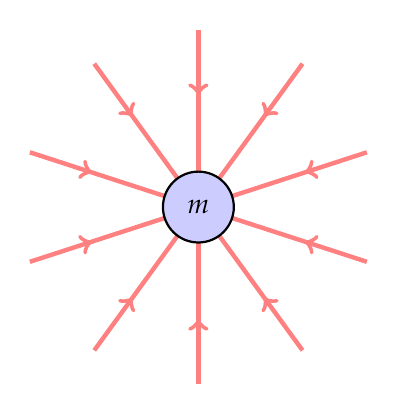
\begin{tikzpicture}[scale=1.5]
      \foreach \x in {0,...,9}\draw[red!50,ultra thick,rotate=36*\x](0,0)--(0,1);
      \foreach \x in {0,...,9}\draw[red!50,<-,ultra thick,rotate around={36*\x:(0,0)}](0,0.95)--(0,1.5);
      \draw[fill=blue!20,thick](0,0) circle(0.3) node{$m$};
    \end{tikzpicture}
  \end{center}
  \begin{itemize}
  \item The direction of $\mb{g}$ is towards the centre of the object that
    created it
  \item Field lines do not tell the intensity (i.e.\ magnitude) of $\mb{g}$,
    only the direction
  \end{itemize}
\end{frame}



\section{Orbital Motion}

\begin{frame}
  \frametitle{Orbital Velocity}
%  \begin{columns}
%    \column{0.75\textwidth}
%    \begin{itemize}
%    \item Substitute $F_\theta$ into Newton's second law, and cancelling mass
%      term, we get:
%
%      \vspace{-0.45in}{\Large
%        \begin{displaymath}
%          F_\theta=ma_\theta\quad\longrightarrow\quad
%          -g\sin\theta=L\frac{d^2\theta}{dt^2}
%        \end{displaymath}
%    }
%    \item For small angles, $\sin\theta\approx\theta$, and we get the ODE for
%      the pendulum:
%      
%      \vspace{-0.2in}{\Large
%        \begin{displaymath}
%          \frac{d^2\theta}{dt^2}+\frac{g}{L}\theta=0
%        \end{displaymath}
%      }
%    \item This ODE has the same form as the mass-spring system!
%    \end{itemize}
%    \column{0.25\textwidth}
%    \begin{tikzpicture}
%      \fill[pattern=north east lines] (-1,0) rectangle (1,0.2);
%      \draw[very thick](-1,0)--(1,0);
%      \begin{scope}[rotate=10]
%        \draw[thick](0,0)--(0,-5);
%        \tikzstyle{balloon}=[ball color=red];    
%        \shade[balloon] (0,-5) circle (0.2) node[below right]{$m$};
%      \end{scope}
%      \draw[dashed,thin](0,0)--(0,-5);
%      \draw[->](0,-2) arc(270:280:2) node[pos=0.5,below]{$\theta$};
%    \end{tikzpicture}
%  \end{columns}
\end{frame}


\begin{frame}
  \frametitle{Orbital Energies}
  \begin{itemize}
  \item Kinetic Energy
%
%    \vspace{-0.25in}{\Large
%      \begin{displaymath}
%        \boxed{\theta(t)=\theta_\mathrm{max}\sin(\omega t+\phi)}
%      \end{displaymath}
%    }
%
%    \vspace{-0.15in}where angular velocity $\omega$ is given by
%    
%    \vspace{-0.15in}{\Large
%      \begin{displaymath}
%        \boxed{\omega=\sqrt{\frac{g}{L}}}
%      \end{displaymath}
%    }
%
%    \vspace{-0.1in} and $\phi$ is a phase shift based on the initial condition
%    of the pendulum.
  \item Gravitational Potential Energy
  \item Total Energy
%    $\theta_\mathrm{max}<\ang{15}$
  \end{itemize}
\end{frame}


\begin{frame}
  \frametitle{Escape Velocity}
%  \textbf{Example 4:} A simple pendulum consists of a mass $m$ attached to a
%  light string of length $l$. If the system is oscillating through small
%  angles, which of the following is true
%  \begin{enumerate}[(a)]
%  \item The frequency is independent of the acceleration due to gravity, $g$.
%  \item The period depends on the amplitude of the oscillation.
%  \item The period is independent of the mass $m$.
%  \item The period is independent of the length $l$.
%  \end{enumerate}
\end{frame}


\begin{frame}
  \frametitle{Kepler's Law of Planetary Motion}
%  \textbf{Example 5:} A bucket full of water is attached to a rope and allowed
%  to swing back and forth as a pendulum from a fixed support. The bucket has a
%  hole in its bottom that allows water to leak out. How does the period of
%  motion change with the loss of water?
%  \begin{enumerate}[(a)]
%  \item The period does not change.
%  \item The period continuously decreases.
%  \item The period continuously increases.
%  \item The period increases to some maximum and then decreases again.
%  \end{enumerate}
\end{frame}


%\begin{frame}
%  \frametitle{Think About $g$}
%  \textbf{Example 6:} A little girl is playing with a toy pendulum while riding
%  in an elevator. Being an astute and educated young lass, she notes that the 
%  period of the pendulum is $T=\SI{0.5}{\second}$. Suddenly the cables
%  supporting the elevator break and all  of the brakes and safety features fail
%  simultaneously. The elevator plunges into free fall. The young girl is
%  astonished to discover that the pendulum has:
%  \begin{enumerate}[(a)]
%  \item continued oscillating with a period of \SI{0.5}{\second}.
%  \item stopped oscillating entirely.
%  \item decreased its rate of oscillation to have a longer period.
%  \item increased its rate of oscillation to have a lesser period.
%  \end{enumerate}
%\end{frame}

\section{Gravitational Potential Energy}


\end{document}
